\documentclass[12pt]{article}
\usepackage[utf8]{inputenc}
\usepackage{graphicx} % Per includere immagini
\usepackage{titling}  % Per personalizzare lo spazio del titolo
\usepackage{ccicons}  % Per i simboli Creative Commons
\usepackage{geometry} % Per personalizzare i margini
\usepackage{hyperref} % Per i link
\usepackage[italian]{babel}
\usepackage{pgffor}
\usepackage{listings}
\usepackage{color}
\usepackage{float}
\usepackage{pdflscape}

\definecolor{codegreen}{rgb}{0,0.6,0}
\definecolor{codegray}{rgb}{0.5,0.5,0.5}
\definecolor{codepurple}{rgb}{0.58,0,0.82}
\definecolor{backcolour}{rgb}{0.95,0.95,0.92}

\lstdefinestyle{mystyle}{
    backgroundcolor=\color{backcolour},   
    commentstyle=\color{codegreen},
    keywordstyle=\color{magenta},
    numberstyle=\tiny\color{codegray},
    stringstyle=\color{codepurple},
    basicstyle=\ttfamily\footnotesize,
    breakatwhitespace=false,         
    breaklines=true,                 
    captionpos=b,                    
    keepspaces=true,                 
    numbers=left,                    
    numbersep=5pt,                  
    showspaces=false,                
    showstringspaces=false,
    showtabs=false,                  
    tabsize=2
}

\lstset{style=mystyle}

% Imposta i margini della pagina
\geometry{
  top=2cm,
  bottom=2cm,
  left=3cm,
  right=3cm
}

\lstset{
  basicstyle=\ttfamily,
  breaklines=true,
  columns=fullflexible
}

\setlength{\droptitle}{-5em} % Sposta in alto il titolo

\title{
    \Large \textbf{UNIVERSITA' DI SALERNO} \\[0.5em]
    \small DIPARTIMENTO DI INGEGNERIA DELL'INFORMAZIONE ED ELETTRICA E MATEMATICA APPLICATA\\[5em]
    
\includegraphics[width=0.6\textwidth]{logo_uni.png}\\[3em] % Logo dell'Università
    \normalsize Laurea Magistrale in Ingegneria Informatica \\[1em]
    \Large \textbf {Project work} \\[1em]
    \large \textbf {Deliverable 3} \\ [1em]
    \large {Sistemi Embedded} \\[1em]
}

\author{
    \textbf{Gruppo: 8} \\
    \normalsize Marotta Giuseppe - 0622702302 - g.marotta31@studenti.unisa.it\\
    \normalsize Rea Gaetano - 0622702190 - g.rea7@studenti.unisa.it\\
    \normalsize Squitieri Giuseppe - 0622702339 - g.squitieri8@studenti.unisa.it\\ 
    \normalsize Tramice Davide - 0622702194 - d.tramice@studenti.unisa.it\\ \\
    }

\date{
    ANNO ACCADEMICO 2023/2024 % Data
}

\begin{document}


\begin{titlingpage} % Crea una pagina di titolo personalizzata
\maketitle
\thispagestyle{empty} % Rimuove il numero di pagina
%\begin{center}
    %\ccbyncnd % Simbolo Creative Commons
%\end{center}
\end{titlingpage}

% Creazione di una nuova pagina
\newpage

% Aggiungi l'indice delle sezioni
\tableofcontents


\newpage

\section{Generazione del codice e implementazione}
In questa sezione verranno presentati i passaggi attuati per effettuare la generazione del codice e il successivo deployment sulla scheda \textbf{STM-32 NUCLEO-G474RE}. Successivamente si è passato ad un intensa campagna di testing direttamente sull'hardware, i risultati sono riportati nell'ultima parte.

\subsection{Il circuito}
Per creare il circuito è stata utilizzata una breadboard che permette di effettuare collegamenti ordinati senza l'utilizzo della saldatrice a stagno. Si è iniziato con il connettere i vari componenti alla breadboard, poi si sono collegate le alimentazioni dei componenti ove necessario ed infine si è collegata la scheda tramite i suoi pin.\\
La configurazione dei pin può essere vista nella successiva tabella:

\vspace{1cm}


\begin{table}[H]
    \centering
    \begin{tabular}{|c|c|c|}
    \hline
    \textbf{Variabile} & \textbf{Pin} & \textbf{Configurazione} 
    \\ \hline
    \texttt{B1} & PC13 & PULL-DOWN \\ \hline
    \texttt{B2} & PC6 & PULL-DOWN  \\ \hline
    \texttt{B3} & PC8 & PULL-DOWN \\ \hline
    \texttt{P1} & PC10 & PULL-UP  \\ \hline
    \texttt{P2} & PC12 & PULL-UP  \\ \hline
    \texttt{RED\_LED} & PB5 & - \\ \hline
    \texttt{YELLOW\_LED} & PB4 & - \\ \hline
    \texttt{GREEN\_LED} & PB3 & - \\ \hline
   \end{tabular}
    \caption{Variabili utilizzate nel modello Stateflow}
    \label{tab:variables}
    \end{table}


\newpage
\subsection{Generazione del codice (Embedded coder)}

Una volta configurata la scheda ed aver accertato che tutti i componenti siano funzionanti si è passato alla generazione del codice tramite il tool \textbf{Embedded coder}. Questo tool permette di generare i file .h e il file .c che descrivono il modello descritto in Simulink.
\begin{itemize}
    \item {\textbf{Setting variabili}} Il primo passaggio effettuato è stato quello che tutte le variabili fossero del tipo giusto, in particolare, le variabili di input e output son di tipo textit{boolean}, mentre le restanti che riguardano i tempi sono di tipo \textit{double}.
    \item {\textbf{Step time}} Successivamente si è scelto lo step time a 0.1 secondi.
    \item {\textbf{Parametri generazione}} A questo punto è stata avviata la generata del codice per un processore \textbf{ARM} di tipo \textbf{Cortex-M}.La generazione produce diversi file, ma quelli che servono sono in particolare 3: \textit{AutomaticGate.h, AutomaticGate.c e rtwtypes.h}.
    \item {\textbf{Import codice}} A questo punto si importano i tre file nel progetto configurato in \textbf{STM32CubeIDE} e si procede alla build del progetto per assicurarsi che i file siano senza errori.
    \item {\textbf{Main}} L'ultima parte da effettuare è quella di configurare il file \textit{main.c}. Nel main sono stati inclusi i file .h importati in precedenza, successivamente sono state create due funzioni per la lettura e la scrittura degli input e degli output ed infine è stata definita la sequenza di azioni da eseguire nel while infinito. Nello snippet di codice successivo è mostrato tutto il codice inserito.
\end{itemize}
\begin{figure}[H]
    \hspace{0.4cm}
    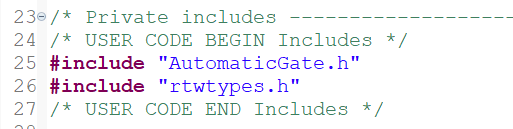
\includegraphics[width=1\textwidth]{snippet/include.png}
    \caption{Include of the system.}
\end{figure}
\begin{figure}[H]
    \hspace{0.72cm}
    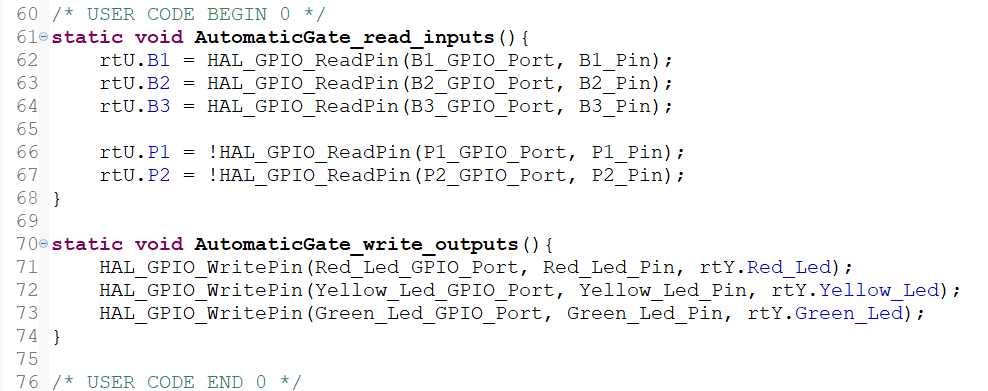
\includegraphics[width=1\textwidth]{snippet/input_output.png}
    \caption{Input and output of the system.}
\end{figure}
\begin{figure}[H]
    \hspace{0.9cm}
    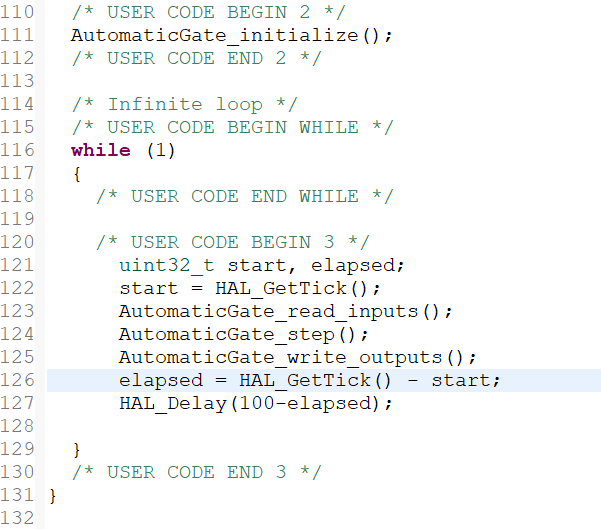
\includegraphics[width=1\textwidth]{snippet/main.png}
    \caption{Testing.}
\end{figure}
\newpage
\subsection{Testing}
Una volta esportato il codice sulla scheda \textbf{STM-32 NUCLEO-G474RE} c'è il bisogno di testare se tutto funzione, in particolare sono stati ripetuti tutti i test eseguiti sul modello, successivamente sono indicati i risultati

\newpage
\addcontentsline{toc}{section}{Elenco delle figure}
\listoffigures
\end{document}
